Una vez definida la escena a partir de un SDF necesitamos una forma para visualizarla, para lo que utilizaremos la API de OpenGL \cite{opengl} y aplicaremos la técnica de \textit{raymarcing}. 

\subsection{Creación del lienzo}
Si bien se puede hacer \textit{raymarching} directamente sobre una escena 3D, nuestra escena constará únicamente de un plano formado por cuatro vértices y dos triángulos, que usaremos como lienzo  (o \textit{canvas}) para dibujar sobre él. Para ello, necesitaremos trabajar sobre diferentes espacios de coordenadas que nos proporciona OpenGL, los cuales pasamos a enumerar.
\begin{itemize}
    \item \textbf{Coordenadas locales o de objeto:} distancias relativas al origen del objeto.
    \item \textbf{Coordenadas globales o de mundo:} distancias relativas a un origen común para todos los objetos.
    \item \textbf{Coordenadas de cámara:} distancias relativas a un sistema de referencia posicionado y alineado con la cámara.
    \item \textbf{Coordenadas de recortado:} distancias normalizadas en el rango $[-1,1]^2$ relativas a un sistema asociado al rectángulo que forma la imagen en pantalla.
\end{itemize}

Para crear el lienzo, debemos declarar sus vértices y cómo estos se unen formando triángulos. Si hacemos uso de \texttt{GL\_TRIANGLES} bastará con definir los vértices en sentido antihorario, pero hay que tener en cuenta que tendremos que repetir dos vértices, ya que se irán formando los triángulos en grupos de tres vértices. Una alternativa para no repetir vértices sería utilizar tablas de vértices e índices, pero en nuestro caso no merece la pena al tener únicamente seis vértices. Un ejemplo de definición de vértices formando un lienzo rectangular podría ser el que se muestra en la \autoref{fig:canvas}.\newline

\begin{figure}[ht]
    \centering
    \begin{minipage}{0.50\textwidth}
        \begin{lstlisting}
glBegin(GL_TRIANGLES);
    glColor3f(1.0f, 1.0f, 1.0f); 
    
    // Triangulo inferior
    glVertex3f(-2.0f, -1.0f, 0.0f);
    glVertex3f(-2.0f, 1.0f, 0.0f);
    glVertex3f(2.0f, 1.0f, 0.0f);
    
    // Triangulo superior
    glVertex3f(-2.0f, -1.0f, 0.0f);
    glVertex3f(2.0f, 1.0f, 0.0f);
    glVertex3f(2.0f, -1.0f, 0.0f);
glEnd();
\end{lstlisting}
    \end{minipage}%
    \hfill
    \begin{minipage}{0.40\textwidth}
        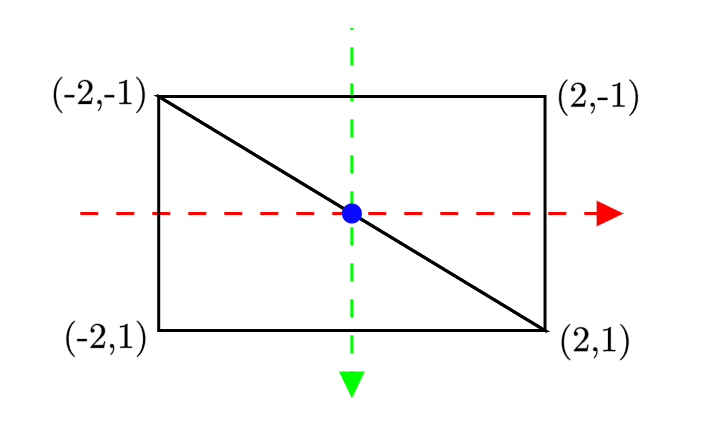
\includegraphics[width=\textwidth]{canvas.png}
    \end{minipage}
    
    
    \caption{Construcción del lienzo}
    \label{fig:canvas}
\end{figure}


Este lienzo, como toda geometría, tendrá asignado dos \textit{shaders} o procesadores, programas escritos en GLSL (lenguaje parecido a C) y que se ejecutan en la GPU. Estos programas son independientes entre sí, y la única forma en la que pueden comunicarse entre ellos es mediante el paso de atributos de entrada y salida con las palabras clave \texttt{in} y \texttt{out} respectivamente. Hay dos tipos de \textit{shaders}: de vértices (\textit{vertex shader}) y de fragmento o píxel (\textit{fragment shader}), cada uno con atributos específicos de entrada y salida.\newline

En el \textit{vertex shader} utilizaremos los siguientes atributos.
\begin{itemize}    
    \item \textbf{\texttt{in vec4 gl\_Vertex}}: contiene las coordenadas locales del vértice actual y es pasado autómaticamente por la aplicación.
    \item \textbf{\texttt{out vec4 gl\_Position}}: posición transformada del vértice actual. La cuarta componente es la componente homogénea, que es necesaria para realizar el cambio a coordenadas recortadas.
\end{itemize}
Por otro lado, en el \textit{fragment shader} usaremos los que siguen.
\begin{itemize}
    \item \textbf{\texttt{in vec4 gl\_FragCoord}}: coordenadas de dispositivo para el centro del píxel actual en el \textit{fragment shader}. Al ser un atributo de entrada del \textit{fragment shader}, está interpolada en cada vértice. La cuarta componente es la inversa de la componente homogénea de \texttt{gl\_Position}, y se utiliza en el cálculo de la profundidad de los píxeles y en las operaciones de corrección de perspectiva.
    \item \textbf{\texttt{out vec4 gl\_FragColor}}: terna RGBA para asignar el color del píxel actual en el \textit{fragment shader}.
\end{itemize}
Por último, en caso de que queramos pasar nuestros propios atributos desde otro programa, deberemos hacerlo a través de un \texttt{uniform}.\newline

En primer lugar se ejecuta el \textbf{procesador de vértices o \textit{vertex shader}} para cada vértice de la geometría. Su objetivo principal es el de realizar transformaciones de coordenadas, y adicionalmente pasar atributos al \textit{fragment shader}. Dada la posición del vértice actual, que se nos proporciona a través del atributo \texttt{gl\_Vertex}, para cambiar de un sistema de coordenadas a otro se utilizan matrices de transformación \cite{article:matrices} \cite{article:matrices2}. En particular, haremos uso de las siguientes.
\begin{figure}[h]
    \centering
    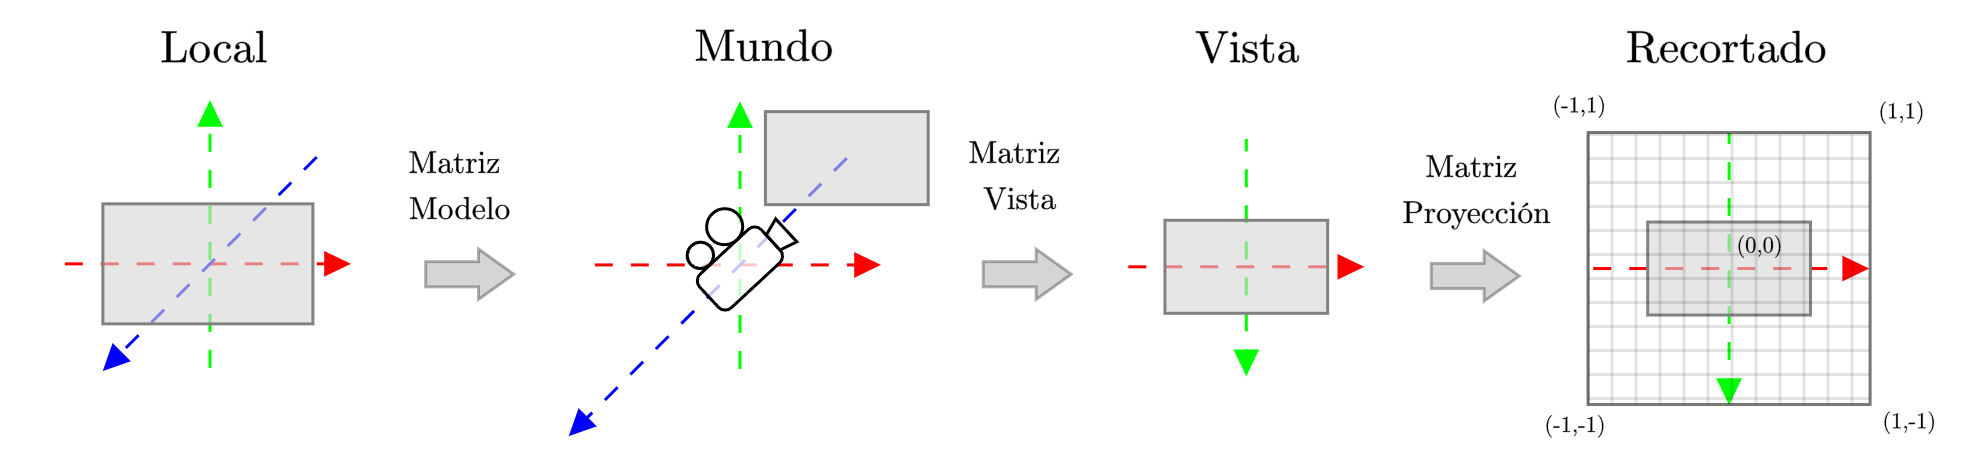
\includegraphics[width=\textwidth]{Plantilla-TFG-master/img/matrices2.png}
    \caption{Coordenadas locales a recortadas}
    \label{fig:matrices}
\end{figure}
\begin{itemize}
    \item \textbf{Matriz de modelo $\boldsymbol{M}$:} define la posición, orientación y escala del objeto en la escena. Se utiliza para pasar del coordenadas locales a coordenadas de mundo. En nuestro caso, si creamos el plano centrado en el origen, podemos simplemente tomar
    \begin{equation*}
        M = Id_{4}.
    \end{equation*}
    \item \textbf{Matriz de vista  $\boldsymbol{V}$:} define la posición y orientación de cada punto respecto a la cámara de la escena. Se utiliza para pasar de coordenadas de mundo a coordenadas de vista. Lo que ocurre en realidad es que la cámara está fija en el origen, y es el resto de la escena es la que se mueve respecto a ella. Por tanto, esta matriz contiene la posición y orientación inversa de la cámara. En nuestro caso, si queremos desplazar la cámara una unidad en el eje Z, la matriz de vista tendrá la forma
    \begin{equation*}
        V = \begin{pmatrix}
        1 & 0 & 0 & 0\\
        0 & 1 & 0 & 0\\
        0 & 0 & 1 & -1\\
        0 & 0 & 0 & 1
        \end{pmatrix}.
    \end{equation*}
    
    \item \textbf{Matriz de proyección:} define cómo la escena se proyecta en la pantalla, incluyendo el campo de visión, aspecto y planos cercano y lejano. Se utiliza para pasar de coordenadas de vista a coordenadas recortadas. OpenGL nos proporciona una función para calcularla como
    \begin{lstlisting}
    glm::mat4 projectionMatrix = glm::perspective(
        glm::radians(FoV),  // campo vertical de vision
        4.0f / 3.0f,         // aspecto
        0.1f,                // plano de corte cercano
        100.0f               // plano de corte lejano
    );
    \end{lstlisting}
    % \item \textbf{Matriz de ventana o \textit{viewport}:} se transforman las coordenadas de recortado a las coordenadas de dispositivo. Estas coordenadas están centradas en la esquina inferior izquierda de la pantalla y están en el rango $[0,r_x]\times [0,r_y]$, donde $r=(r_x,r_y)$ es la resolución de la pantalla.
\end{itemize}

Con esto, ya podemos escribir nuestro \textit{vertex shader}:
\begin{figure}[ht!]
    \centering
       \begin{algorithm}[H]
            \caption{Fragment Shader}
            \KwData{matriz de proyección $M_P$, matriz de vista $M_V$, matriz de modelo $M_M$}
            \KwResult{Posición transformada del vértice actual}
                $gl\_Position \gets M_P \cdot M_V \cdot M_M \cdot gl\_Vertex$
        \end{algorithm}
    \caption{Cuerpo del método \texttt{main} del \textit{vertex shader}}
    \label{fig:mainVS}
\end{figure}

Tras realizar estas transformaciones, las coordenadas de recortado se transforman a coordenadas de dispositivo, que están centradas en la esquina inferior izquierda de la pantalla y toman valor en el rango $[0,r_x]\times [0,r_y]$, donde $r=(r_x,r_y)$ es la resolución de la pantalla.\newline

Ahora le toca el turno al \textbf{procesador de fragmentos o \textit{fragment shader}}. Este se ejecuta para cada píxel de la pantalla, y su objetivo es asignar a la variable \texttt{gl\_FragColor} el color que el píxel tendrá como una terna RGBA. Será aquí donde hagamos todos los cálculos necesarios pare renderizar la superficie con \textit{raymarching}. Para ello, necesitaremos un sistema de coordenadas dentro del propio lienzo, que generaremos haciendo uso de \texttt{gl\_FragCoord} y la resolución del lienzo, atributo que pasaremos nosotros al \textit{shader} a través de un \texttt{uniform}, que llamaremos \texttt{u\_resolution}.\newline

Para obtener estas coordenadas, primero desplazamos el origen que nos proporciona \texttt{gl\_FragCoord} al centro de la pantalla, y posteriormente normalizamos respecto a alguno de los ejes. Hacemos esto porque si intentamos normalizar sobre ambos ejes, obtendremos coordenadas en el rango $[-0.5,0.5]^2$, lo que hará que en un lienzo que no sea cuadrado, la imagen se vea estirada en la dirección del eje más largo. Nosotros normalizaremos respecto al eje vertical, ya que en nuestro caso será siempre el menor. Esto nos dará como resultado unas coordenadas con valores en $\left[ -0.5\cdot aspect, 0.5\cdot aspect \right] \times [-0.5, 0.5]$, donde $aspect$ es el ratio de aspecto del lienzo. Finalmente, para que el eje vertical toma valores en $[-1,1]$ multiplicamos por $2$, obteniendo
\begin{equation*}
    uv = \frac{2\cdot(gl\_FragCoord.xy - 0.5\cdot u\_resolution.xy)}{u\_resolution.y}.
\end{equation*}

Hemos denotado a las coordenadas obtenidas como \texttt{uv}, haciendo referencia a la similitud que tienen con el uso que se le da a las coordenadas de textura habituales. Podemos ver la diferencia entre ambos sistemas de coordenadas si usamos \texttt{uv} como los canales rojo y verde de \texttt{gl\_FragColor}, tal y como se muestra en la \autoref{fig:uv} (los valores que se salen del rango $[-1,1]$ son visualizados como si hubieran sido acotados en dicho intervalo).\newline

\begin{figure}[htbp]
    \centering
    \begin{minipage}[b]{0.45\textwidth}
        \centering
        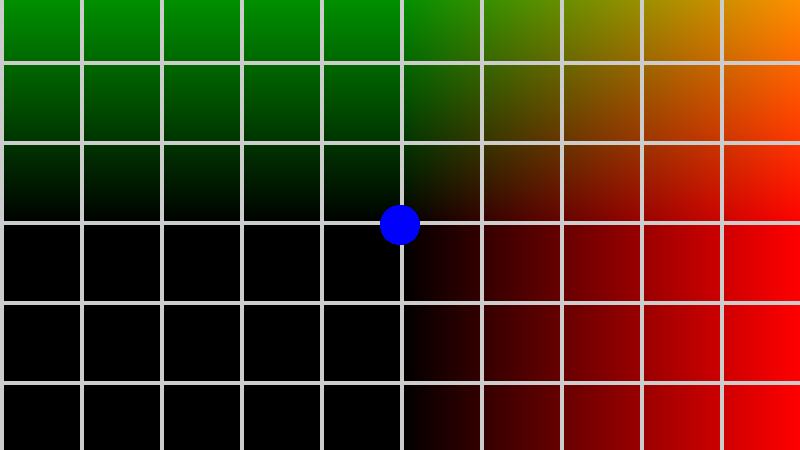
\includegraphics[width=\textwidth]{Plantilla-TFG-master/img/normX.png}
        \caption{Eje X}
    \end{minipage}
    \hfill
    \begin{minipage}[b]{0.45\textwidth}
        \centering
        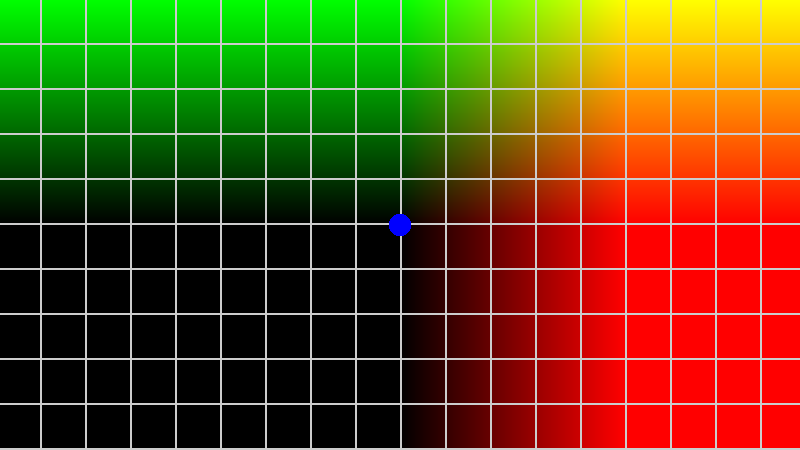
\includegraphics[width=\textwidth]{Plantilla-TFG-master/img/normY.png}
        \caption{Eje Y}
    \end{minipage}
    
    \medskip
    
    \begin{minipage}[b]{0.45\textwidth}
        \centering
        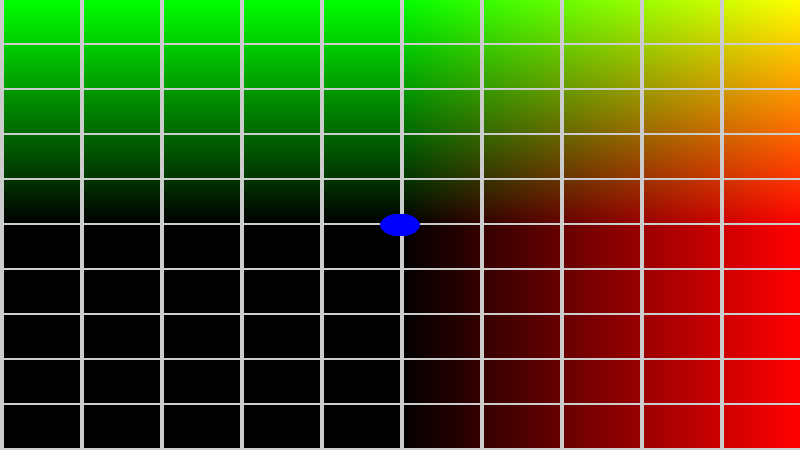
\includegraphics[width=\textwidth]{Plantilla-TFG-master/img/normXY.png}
        \caption{Ejes X e Y}
    \end{minipage}
    
    \caption{Normalización de coordenadas sobre distintos ejes}
    \label{fig:uv}
\end{figure}

Veamos  cómo usar estas coordenadas para dibujar nuestra superficie sobre el lienzo.

\subsection{Raymarching y spheretracing}\label{sec:tracing}
A partir de ahora, pensamos en que nuestra escena no es la de OpenGL, sino aquella que queremos dibujar usando \textit{raymarching} dado un SDF $\phi$. Podemos pensar en esta escena como $\R^3$ con su base usual $B_u = \{e_x,e_y,e_z\} = \{(1,0,0),(0,1,0),(0,0,1)\}$, donde colocamos los siguientes elementos.
\begin{itemize}
    \item La \textbf{isosuperficie} $S_{\phi}$.
    \item \textbf{Plano de visión:} rejilla perpendicular al eje óptico de la cámara, donde cada uno de sus cuadrados corresponde a un píxel del lienzo.
    \item \textbf{Punto de la cámara $\boldsymbol{c_o}$:} punto del espacio desde donde se observa la escena.
    \item \textbf{Punto de atención o \textit{lookat point} $\boldsymbol{l}$:} hacia que punto del espacio debe mirar la cámara. En general tomaremos $l=(0,0,0)$.
\end{itemize}

El método del \textit{raymarching} consiste en trazar rayos a partir de $c_o$ hacia el centro de cada uno de los cuadrados del plano de visión, de forma que si el rayo interseca con $S_\phi$ significa que ese píxel corresponde a un punto de la superficie, y será coloreado como tal.
\begin{figure}[h]
    \centering
    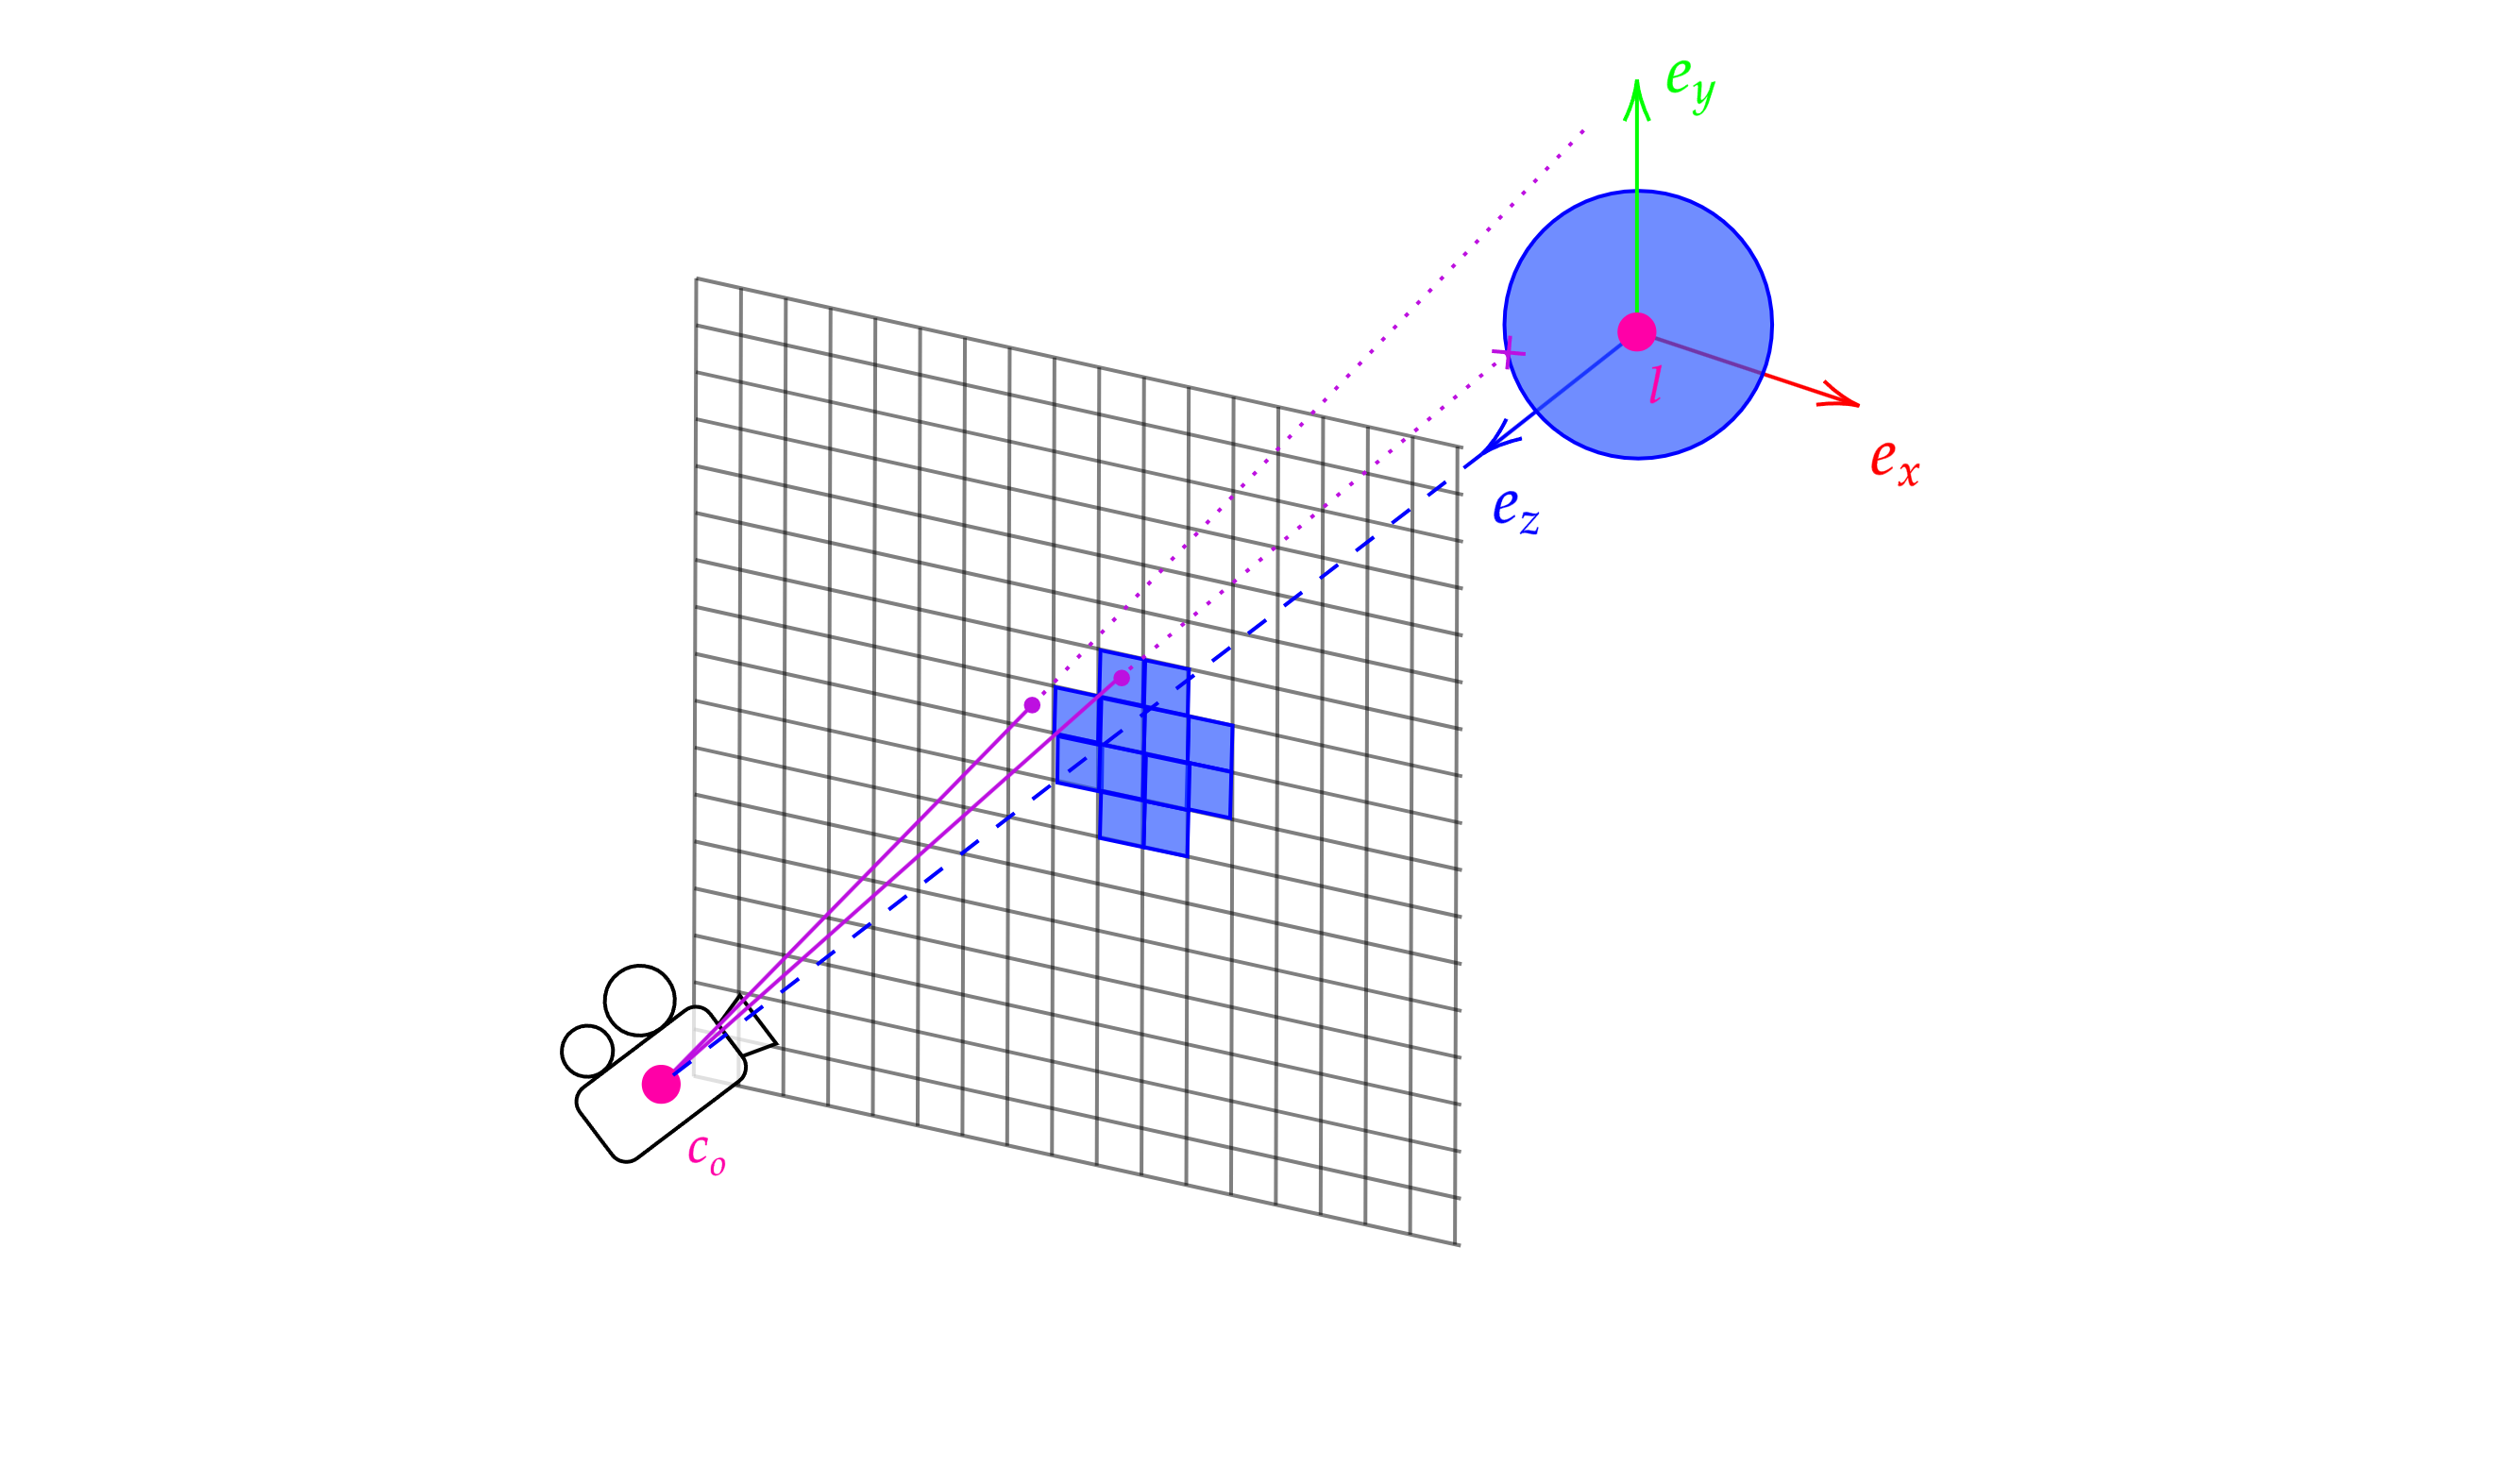
\includegraphics[width=\textwidth]{Plantilla-TFG-master/img/raymarch_fix.png}
    \caption{Trazado de rayos a través del plano de visión}
    \label{fig:raymarch1}
\end{figure}
\newline

Cada uno de estos rayos estará definido por un origen $r_o$ y una dirección $r_d$. El origen será siempre la posición de la cámara $c_o$, pero la dirección requiere más trabajo. En el escenario descrito en la \autoref{fig:raymarch1} en el que $S_{\phi}$ es una esfera centrada en el origen y el observador se encuentra sobre el eje Z, dado que en todo momento conocemos las coordenadas de cada punto de la rejilla a través de $uv = (u,v)$, es claro que podemos tomar
$$r_d = (u,v,0) - c_0.$$ 
Tomando $c_0 = (0,0,c)$, el valor $c$ actuaría como un control del campo de visión, de forma que cuanto menor sea su valor, menor se verán los objetos dibujados. Lo fijaremos a un valor de $1$. Sin embargo este escenario es el más sencillo posible, y si queremos poder mover la cámara manteniendo la orientación hacia $l$ tendremos que poder trabajar con  orientación arbitraria suya. Para ello deberemos construir un marco cartesiano relativo a la cámara, esto es, una base $B=\{f_1,f_2,f_3\}$ de $\R^3$ alineada con ella. Esta base deberá ser ortonormal y tener la misma orientación que la base usual.\newline

Obtenemos primero vectores que nos resultarán útiles para generar esta base.

\begin{itemize}
    \item \textbf{Vector director $\boldsymbol{c_d}$:} indica la dirección hacia la que mirará la cámara. luego vendrá dado por $c_d = l-c_o$.
    \item \textbf{\textit{Right vector} $\boldsymbol{c_r}$ }: es el análogo a $e_x$ en la base usual, luego lo podemos obtener como $c_r = (0,1,0)\times c_d$.
    \item \textbf{\textit{Up vector} $\boldsymbol{c_u}$}: dirección en la que el observador ve proyectada en vertical la escena. Podemos obtenerlo como $c_u = c_d\times c_r$.
\end{itemize}

A partir de estos vectores podemos obtener $\{f_1,f_2,f_3\}$ normalizándolos y teniendo en cuenta que el plano de visión y la cámara estarán orientados de forma opuesta:
\begin{equation*}
    f_1 = -\frac{c_r}{\Vert c_r\Vert} = -\frac{(0,1,0)\times c_d}{\Vert l-c_o\Vert},\quad 
    f_2 = \frac{c_u}{\Vert c_u\Vert } = f_3\times f_1, \quad
    f_3 = -\frac{c_d}{\Vert c_d\Vert} = -\frac{l-c_o}{\Vert l-c_o\Vert}. 
\end{equation*}

Solo queda transformar el vector $r_d = (u,v,-1)$ a la base que acabamos de obtener. La matriz de cambio de base serán las coordenadas por columnas de $\{f_1,f_2,f_3\}$ escritas en función de $\{e_1,e_2,e_3\}$, que al ser la base usual, coincidirá con escribir por columnas $\{f_1,f_2,f_3\}$, de forma que
\begin{equation*}
    rayo = (u,v,-1)_{B}^t = \big(f_1\ \vert\  f_2\  \vert\  f_3\big) \cdot \begin{pmatrix}
        u\\
        v\\
        -1
    \end{pmatrix}.
\end{equation*}

\begin{figure}[ht!]
    \centering
    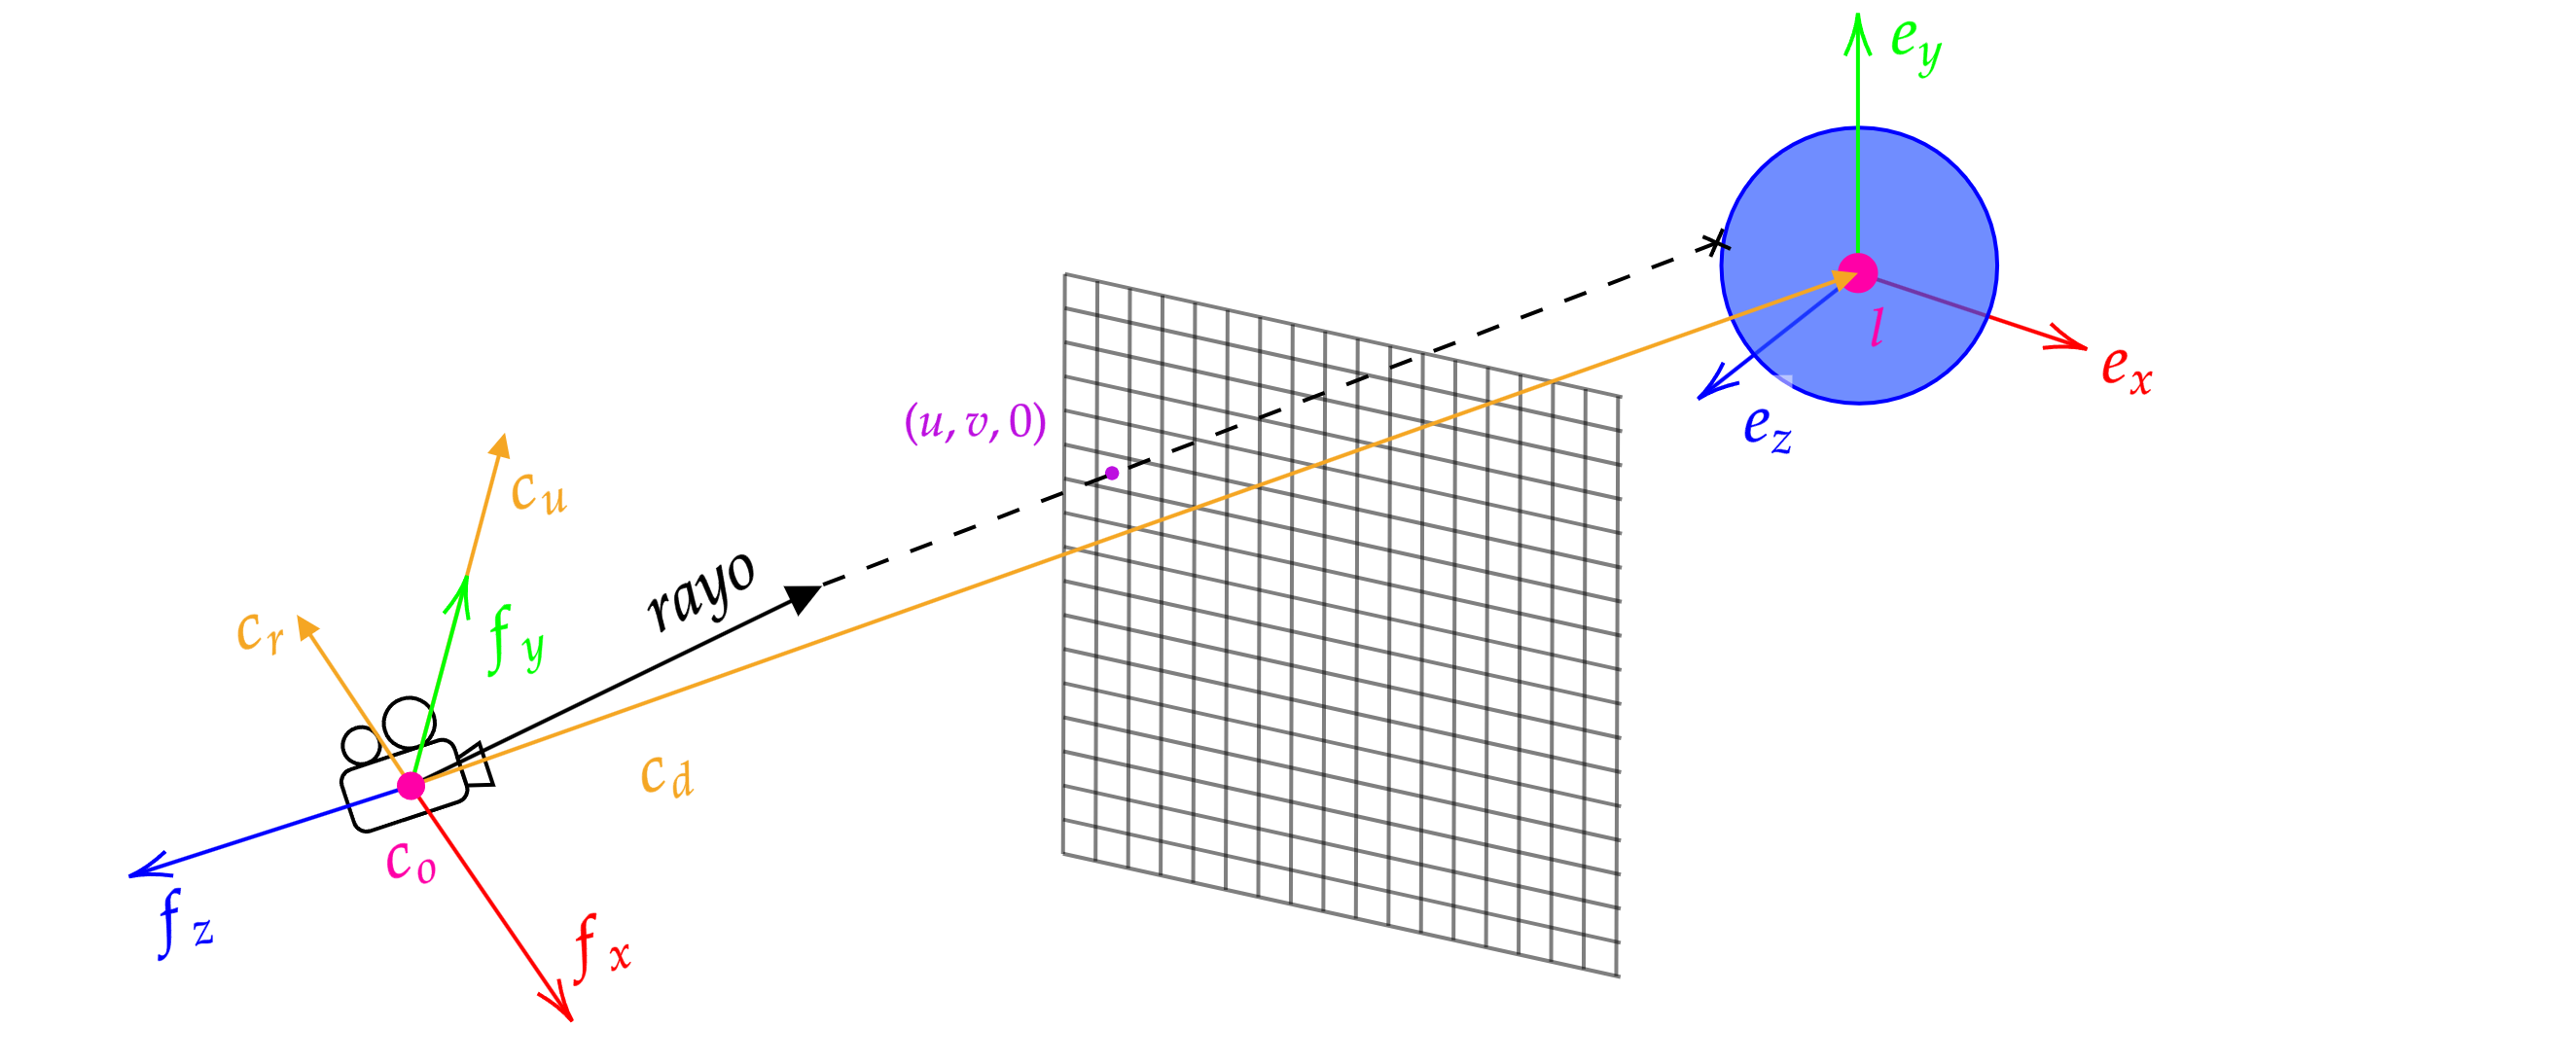
\includegraphics[width=\textwidth]{Plantilla-TFG-master/img/raydir_fix.png}
    \caption{Obtención de la dirección del rayo}
    \label{fig:raydir}
\end{figure}

Ahora que ya tenemos toda la información del rayo, falta comprobar si este interseca con $S_{\phi}$. Para esto se utiliza un método iterativo: a partir de $c_o$, en cada iteración avanzamos en la dirección del rayo una distancia fija $\delta$. Evaluamos entonces nuestro SDF en la posición actual, de forma que si obtenemos un valor muy cercano a $0$ significará que hemos llegado a la isosuperficie. De lo contrario, repetimos el proceso hasta encontrar una intersección o superar un número máximo de iteraciones, en cuyo caso concluiremos que no hay intersección. La \autoref{a:raymarching} ilustra este procedimiento, donde \texttt{DibujarSuperficie()} y \texttt{DibujarFondo()} devuelven ternas RGBA que serán asignadas al píxel actual dependiendo de si hay intersección o no.\newline

\begin{figure}[ht!]
    \centering
    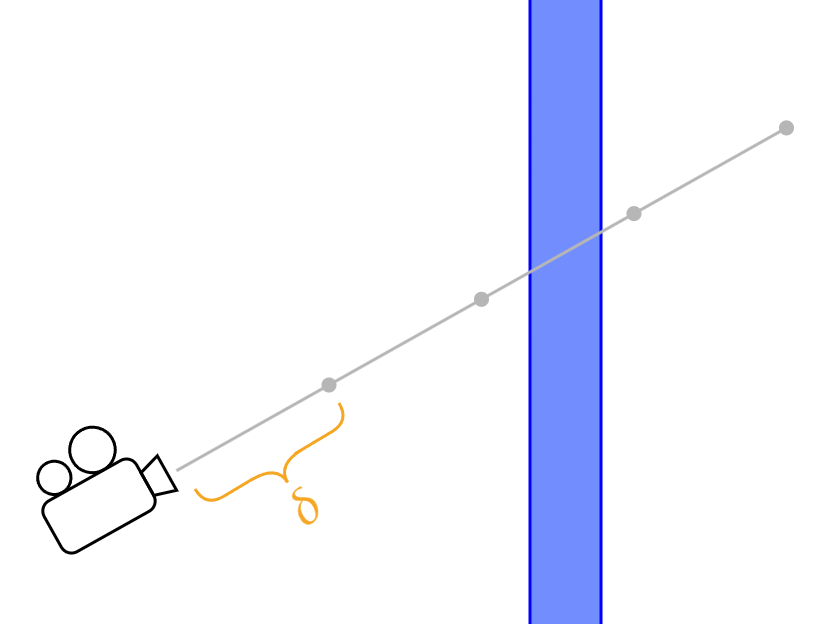
\includegraphics[width=0.4\textwidth]{Plantilla-TFG-master/img/miss.png}
    \caption{Pérdida de intersección en \textit{raymarching} para valores elevados de $\delta$}
    \label{fig:miss}
\end{figure}

\SetKwComment{Comment}{// }{}
\begin{figure}[ht!]
    \centering
    \begin{minipage}{0.50\textwidth}
        \begin{algorithm}[H]
            \caption{Raymarching}
                \KwData{origen $c_o$, dirección $v$}
                \KwResult{Terna RGB con el color asignado al píxel actual}
                
                $d \gets 0$ \Comment{distancia total}
                
                \For{i $\in$ MAX\_ITERACIONES} {
                    $p \gets c_o +d\cdot v$
                    
                    sdf $\gets \phi(\text{p})$
                    
                    \If{sdf $< \varepsilon$}{
                       \Return{DibujarSuperficie($p,v,sdf$)}
                    }
            
                    $d\gets d + \delta$\;
            
                    \If{$d >$ MAX\_DISTANCIA}{
                        \Return{DibujarFondo()}
                    }
                }
        \end{algorithm}
    \end{minipage}%
    \hfill
    \begin{minipage}{0.48\textwidth}
        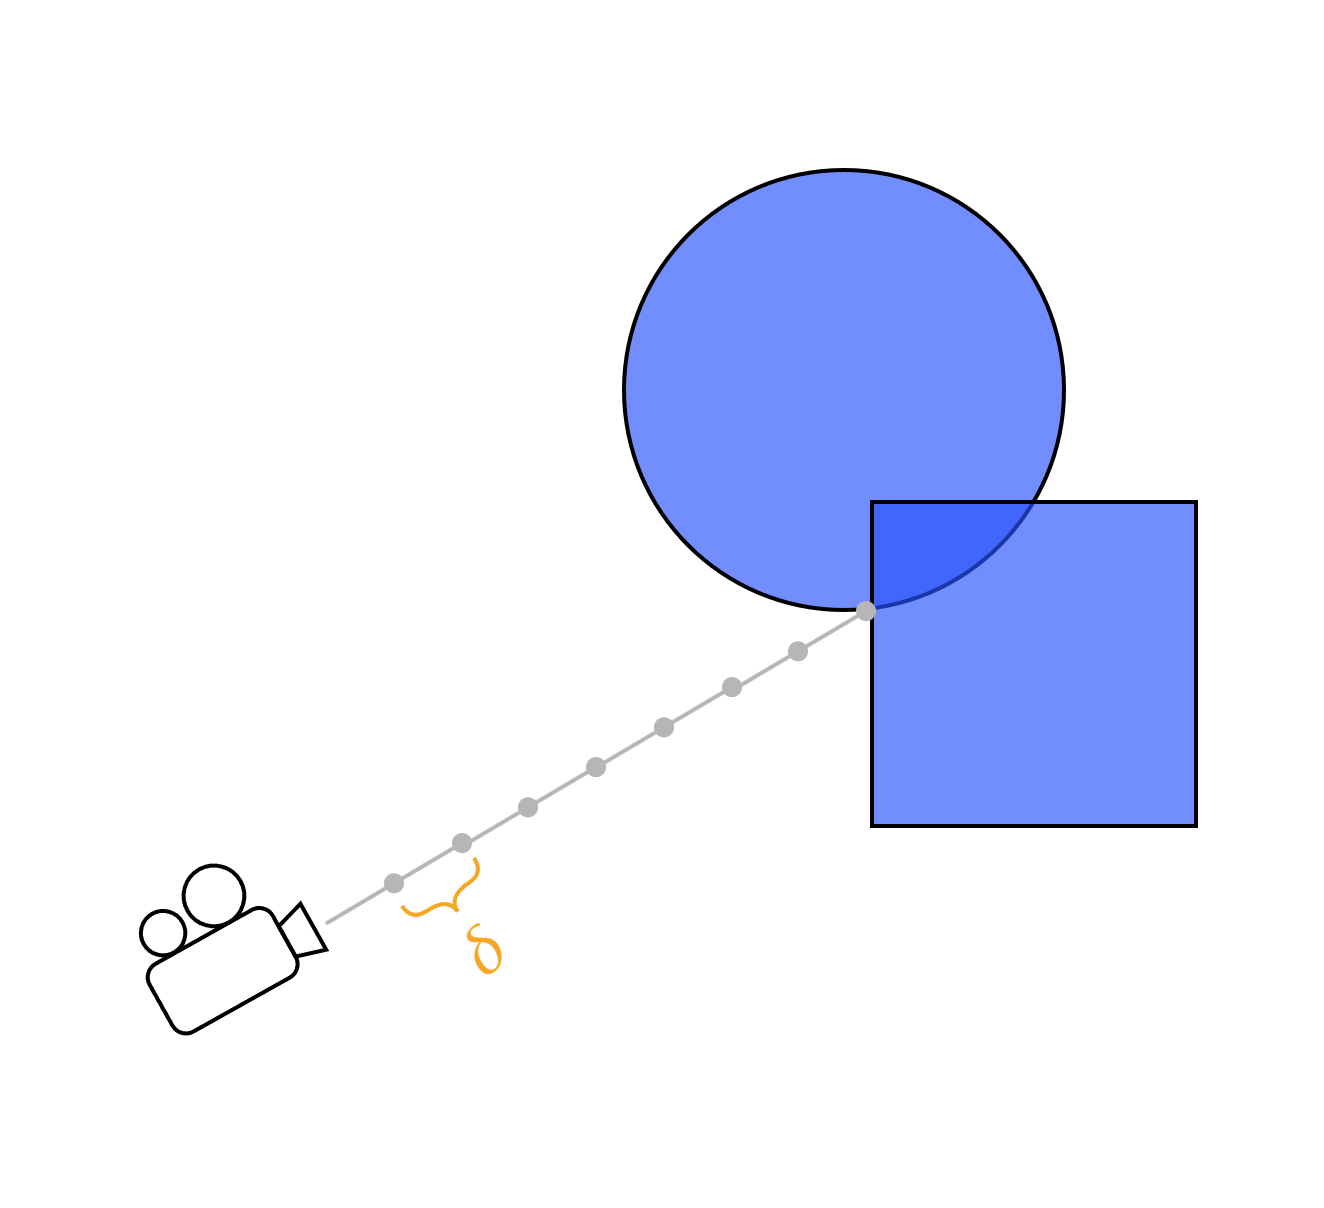
\includegraphics[width=\textwidth]{raymarching.png}
    \end{minipage}
    \caption{Algoritmo de \textit{raymarching}}
    \label{a:raymarching}
\end{figure}

Una desventaja de esta técnica es que puede ser bastante lenta, ya que cuanto más alejados estén los puntos de $S_\phi$ del observador, mayor es el número de iteraciones necesarias para encontrar la intersección en caso de que la haya. En el peor de los casos en el que tal intersección no exista, se habrá realizado el número máximo de iteraciones, que deberá ser bastante alto, pues si no queremos perder ninguna intersección como ocurre en la \autoref{fig:miss}, el valor de incremento $\delta$ tenddrá que ser pequeño.\newline

La solución a este problema es el uso de \textit{spheretracing}, que reduce drásticamente el número de iteraciones y por tanto evaluaciones de $\phi$, necesarias para detectar la intersección. Su funcionamiento es similar al \textit{raymarching}, con la diferencia de que el incremento en la posición del rayo no es fija, sino que es la máxima que podemos tomar en cada momento asegurándonos de no perder información. Esta distancia será la mínima del punto actual del rayo a $S_\phi$, que no es más que evaluar $\phi$ en dicho punto.\newline

Este será por tanto el algoritmo que utilizaremos para detectar qué píxeles de la pantalla corresponden a la superficie $S_{\phi}$, y se encuentra descrito con detalle en la \autoref{a:spheretracing}. 
Con esto al fin podemos describir la forma que tendrá nuestro \textit{fragment shader} en la \autoref{fig:mainFS}. Claro está que esta versión todavía no es funcional, pues no sabemos qué forma tiene \texttt{DibujarSuperficie}, y como mucho podremos obtener una imagen que separe la isosuperficie del fondo usando colores planos como muestra la \autoref{fig:planos} para una esfera centrada en el origen. Veremos como mejorar esto en la próxima sección.

\begin{figure}[ht!]
    \centering
    \begin{minipage}{0.50\textwidth}
       \begin{algorithm}[H]
            \caption{Spheretracing}
                \KwData{origen $c_o$, dirección $v$}
                \KwResult{Terna RGB con el color asignado al píxel actual}
                $d \gets 0$ \Comment{distancia actual}
                
                \For{i $\in$ MAX\_ITERACIONES} {
                    $p \gets c_o + d \cdot v$
                    
                    sdf $\gets \phi(p)$
                    
                    \If{sdf $< \varepsilon$}{
                       \Return{DibujarSuperficie($p,v,sdf$)};
                    }
            
                    $d \gets$ d + sdf
            
                    \If{$d >$ MAX\_DISTANCIA}{
                        \Return{DibujarFondo()};
                    }
                }
        \end{algorithm}
    \end{minipage}%
    \hfill
    \begin{minipage}{0.48\textwidth}
        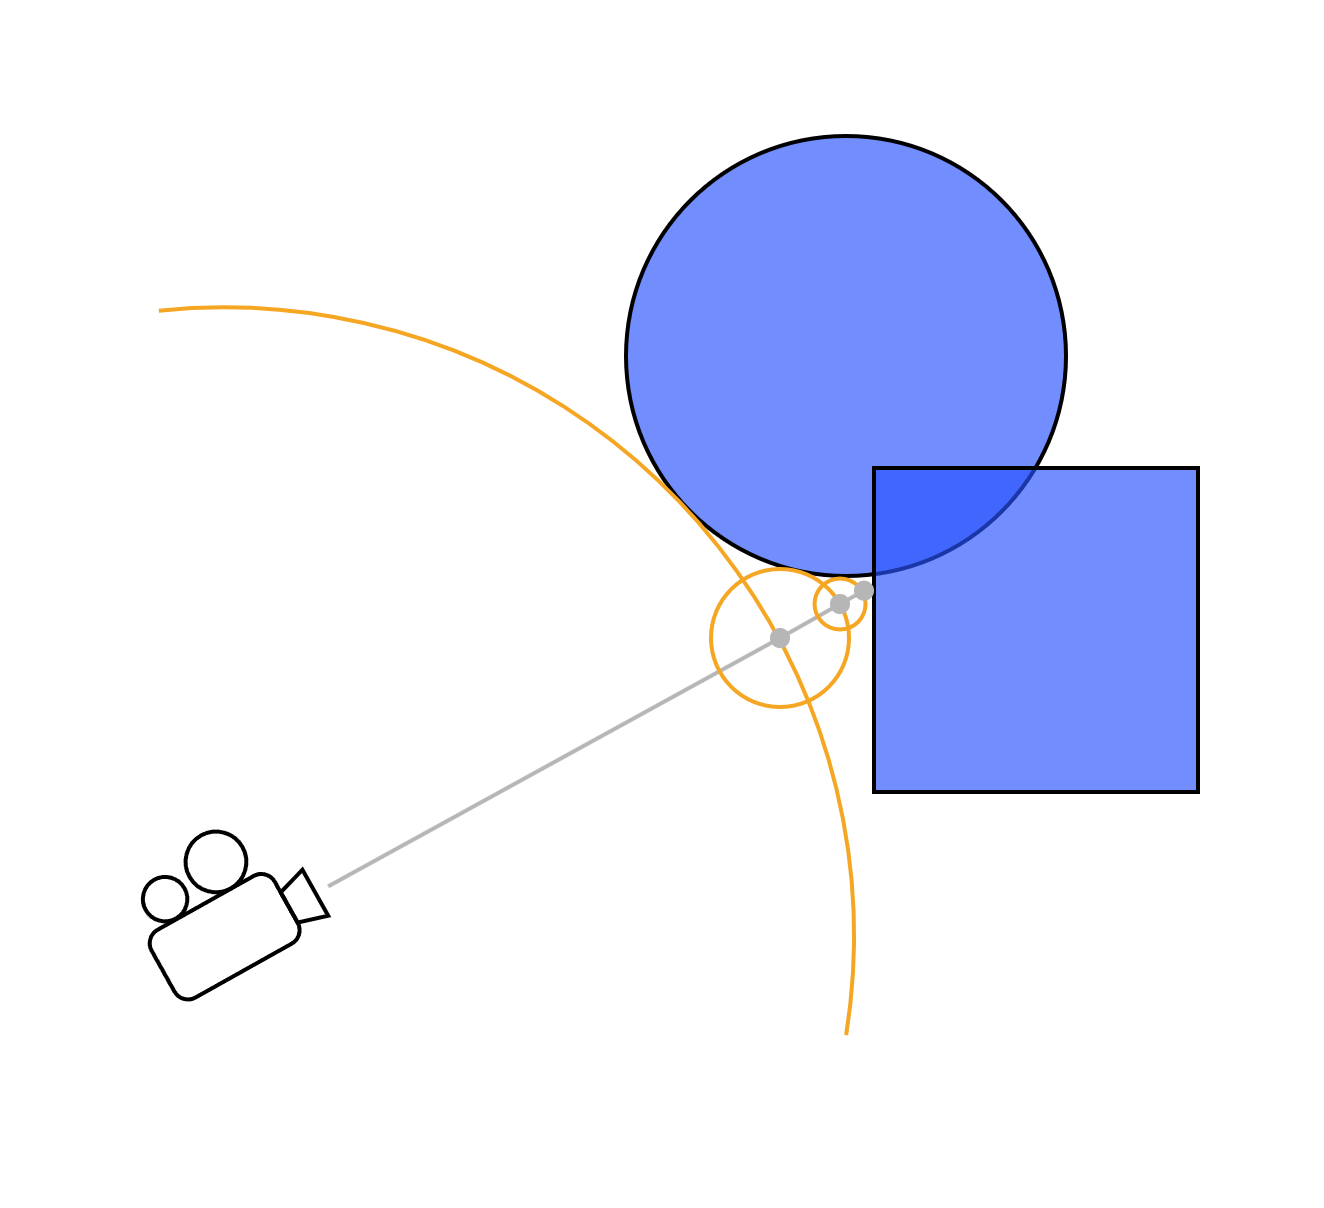
\includegraphics[width=\textwidth]{spheremarching.png}
    \end{minipage}
    \caption{Algoritmo de \textit{spheretracing}}
    \label{a:spheretracing}
\end{figure}

\begin{figure}[ht!]
    \centering
    
       \begin{algorithm}[H]
            \caption{Fragment Shader}
            \KwData{posición del observador $c_0$, punto de atención $l$}
            \KwResult{Terna RGBA con el color asignado al píxel actual}
            
                $uv \gets 2\cdot \frac{gl\_FragCoord.xy- 0.5\cdot u\_resolution.xy}{u\_resolution.y}$\\[8pt]

                $r_d \gets (f_1\ \vert \ f_2\ \vert \ f_3)\cdot normalizar((uv.xy,-1))$\\[5pt]

                $color \gets spheretracing(c_0, r_d)$\\[5pt]

                $gl\_FragColor = (color, 1)$
        \end{algorithm}
    \caption{Cuerpo del método \texttt{main} del \textit{fragment shader}}
    \label{fig:mainFS}
\end{figure}


\begin{figure}[ht!]
    \centering
    
\includegraphics[width=0.8\textwidth]{Plantilla-TFG-master/img/escenaPlana.png}
    \caption{Resultado de \textit{spheretracing} asignando colores planos}
    \label{fig:planos}
\end{figure}
